%% CE49X - Lecture 07: Introduction to Machine Learning
%% Fall 2025
%% Instructor: Dr. Eyuphan Koc
%% Bogazici University

\documentclass[10pt,aspectratio=169]{beamer}

%% ==================== PACKAGES ====================
\usepackage[utf8]{inputenc}
\usepackage[T1]{fontenc}
\usepackage{amsmath,amssymb,amsfonts,amsthm}
\usepackage{graphicx}
\usepackage{hyperref}
\usepackage{tikz}
\usepackage{pgfplots}
\pgfplotsset{compat=1.17}
\usetikzlibrary{positioning,arrows.meta,calc,trees,patterns,decorations.pathreplacing,shapes}
\usepackage{booktabs}
\usepackage{array}
\usepackage{multicol}
\usepackage{listings}

%% ==================== THEME SETUP ====================
\usetheme{Madrid}
\usecolortheme{default}

%% Define custom colors
\definecolor{bunavy}{RGB}{0,20,60}
\definecolor{lightgray}{RGB}{245,245,245}
\definecolor{mediumgray}{RGB}{200,200,200}
\definecolor{darkgray}{RGB}{80,80,80}
\definecolor{softred}{RGB}{180,60,60}
\definecolor{softgreen}{RGB}{60,120,60}
\definecolor{softblue}{RGB}{100,140,180}
\definecolor{pythonblue}{RGB}{55,118,171}
\definecolor{pythonyellow}{RGB}{255,212,59}
\definecolor{codegreen}{RGB}{0,128,0}
\definecolor{codepurple}{RGB}{128,0,128}

%% Beamer color theme
\setbeamercolor{structure}{fg=bunavy}
\setbeamercolor{frametitle}{fg=white,bg=bunavy}
\setbeamercolor{title}{fg=white,bg=bunavy}
\setbeamercolor{block title}{bg=mediumgray,fg=darkgray}
\setbeamercolor{block body}{bg=lightgray,fg=black}
\setbeamercolor{block title example}{fg=white,bg=softblue}
\setbeamercolor{block body example}{fg=black,bg=softblue!10!white}
\setbeamercolor{block title alerted}{fg=white,bg=softred}
\setbeamercolor{block body alerted}{fg=black,bg=softred!5!white}

%% Remove navigation symbols
\setbeamertemplate{navigation symbols}{}
\setbeamertemplate{blocks}[rounded][shadow=false]

%% Reduce font sizes and spacing
\setbeamerfont{frametitle}{size=\large}
\setbeamerfont{framesubtitle}{size=\normalsize}
\setbeamerfont{block title}{size=\small}
\setbeamerfont{block body}{size=\small}

%% Reduce list spacing
\setbeamertemplate{itemize/enumerate body begin}{\small}
\setbeamertemplate{itemize/enumerate subbody begin}{\small}
\setlength{\leftmargini}{0.8em}
\setlength{\leftmarginii}{0.6em}
\setlength{\itemsep}{1pt}
\setlength{\parskip}{1pt}
\setlength{\parsep}{0pt}
\setlength{\topsep}{2pt}
\setlength{\partopsep}{1pt}

%% Reduce block spacing
\addtobeamertemplate{block begin}{\vspace*{-2pt}}{}
\addtobeamertemplate{block end}{}{\vspace*{-2pt}}
\setlength{\abovecaptionskip}{2pt}
\setlength{\belowcaptionskip}{2pt}

%% Tighten math displays
\AtBeginDocument{%
  \setlength{\abovedisplayskip}{3pt}%
  \setlength{\belowdisplayskip}{3pt}%
  \setlength{\abovedisplayshortskip}{2pt}%
  \setlength{\belowdisplayshortskip}{2pt}%
}

%% Fix frame numbering
\setbeamertemplate{footline}{
  \leavevmode%
  \hbox{%
  \begin{beamercolorbox}[wd=.333333\paperwidth,ht=2.25ex,dp=1ex,center]{author in head/foot}%
    \usebeamerfont{author in head/foot}\insertshortauthor~~(\insertshortinstitute)
  \end{beamercolorbox}%
  \begin{beamercolorbox}[wd=.333333\paperwidth,ht=2.25ex,dp=1ex,center]{title in head/foot}%
    \usebeamerfont{title in head/foot}\insertshorttitle
  \end{beamercolorbox}%
  \begin{beamercolorbox}[wd=.333333\paperwidth,ht=2.25ex,dp=1ex,right]{date in head/foot}%
    \usebeamerfont{date in head/foot}\insertshortdate{}\hspace*{2em}
    \insertframenumber{} / \inserttotalframenumber\hspace*{2ex}
  \end{beamercolorbox}}%
  \vskip0pt%
}

%% ==================== CODE LISTING SETUP ====================
\lstset{
    language=Python,
    basicstyle=\ttfamily\tiny,
    keywordstyle=\color{codepurple}\bfseries,
    commentstyle=\color{codegreen},
    stringstyle=\color{softred},
    numberstyle=\tiny\color{mediumgray},
    numbers=left,
    numbersep=5pt,
    xleftmargin=15pt,
    xrightmargin=5pt,
    framexleftmargin=0pt,
    breaklines=true,
    breakatwhitespace=true,
    frame=single,
    backgroundcolor=\color{lightgray},
    showspaces=false,
    showstringspaces=false,
    tabsize=4,
    captionpos=b
}

%% ==================== CUSTOM COMMANDS ====================
% Machine Learning notation
\newcommand{\X}{\mathbf{X}}
\newcommand{\y}{\mathbf{y}}
\newcommand{\w}{\mathbf{w}}
\newcommand{\xvec}{\mathbf{x}}
\newcommand{\yvec}{\mathbf{y}}
\DeclareMathOperator*{\argmin}{argmin}
\DeclareMathOperator*{\argmax}{argmax}
\newcommand{\R}{\mathbb{R}}
\newcommand{\E}{\mathbb{E}}

% Inline code
\newcommand{\py}[1]{\texttt{#1}}
\newcommand{\pyvar}[1]{\textcolor{pythonblue}{\texttt{#1}}}
\newcommand{\pykeyword}[1]{\textcolor{codepurple}{\textbf{\texttt{#1}}}}

\AtBeginSection[]
{
  \begin{frame}
    \frametitle{Outline}
    \tableofcontents[currentsection]
  \end{frame}
}

%% ==================== TITLE INFORMATION ====================
\title[CE49X - Week 7]{CE49X: Introduction to Machine Learning}
\subtitle{Foundations of Machine Learning with Scikit-Learn}
\author[Dr. E. Koc]{Dr. Eyuphan Koc}
\institute[BU]{
  Department of Civil Engineering\\
  Bogazici University
}
\date{Fall 2025}

%% ==================== DOCUMENT ====================
\begin{document}

%% Title Slide
\begin{frame}[plain]
  \titlepage
  \begin{center}
    \vspace{0.3cm}
    \footnotesize
    Based on \textit{Python Data Science Handbook} by Jake VanderPlas\\
    Chapter 5: Machine Learning (Sections 5.0--5.6)\\
    \url{https://jakevdp.github.io/PythonDataScienceHandbook/}
  \end{center}
\end{frame}

%% Table of Contents
\begin{frame}{Lecture Outline}
\small
  \tableofcontents
\end{frame}

%% ==================== SECTION 1: WHAT IS MACHINE LEARNING ====================
\section{What is Machine Learning?}

\begin{frame}{What is Machine Learning?}
\small
\textbf{Definition:}
\begin{itemize}
\item Machine Learning is about building \textbf{mathematical models} to understand data
\item Fundamentally, it's a \textbf{data-driven approach} to learning patterns
\item Models learn from examples rather than explicit programming
\end{itemize}

\vspace{0.2cm}
\textbf{Key Idea:}
\begin{quote}
\textit{"Instead of programming explicit rules, we provide examples and let the algorithm discover the patterns."}
\end{quote}

\vspace{0.2cm}
\begin{exampleblock}{Civil Engineering Example}
Rather than coding rules for predicting concrete strength, we provide examples of mix designs and their measured strengths—the model learns the relationship.
\end{exampleblock}
\end{frame}

\begin{frame}{Categories of Machine Learning}
\small
\begin{columns}[T]
\column{0.48\textwidth}
\textbf{Supervised Learning}
\begin{itemize}
\item Learn from \textbf{labeled} data
\item Have input-output pairs
\item Goal: predict outputs for new inputs
\end{itemize}

\vspace{0.1cm}
\textbf{Two Types:}
\begin{enumerate}
\item \textcolor{softblue}{\textbf{Classification}}: Predict discrete labels
\item \textcolor{softgreen}{\textbf{Regression}}: Predict continuous values
\end{enumerate}

\column{0.48\textwidth}
\textbf{Unsupervised Learning}
\begin{itemize}
\item Learn from \textbf{unlabeled} data
\item No predefined outputs
\item Goal: discover structure
\end{itemize}

\vspace{0.1cm}
\textbf{Two Types:}
\begin{enumerate}
\item \textcolor{softblue}{\textbf{Clustering}}: Group similar items
\item \textcolor{softgreen}{\textbf{Dimensionality Reduction}}: Compress data
\end{enumerate}
\end{columns}

\vspace{0.3cm}
\begin{alertblock}{Key Difference}
Supervised: ``Here are examples with answers'' vs Unsupervised: ``Find patterns in this data''
\end{alertblock}
\end{frame}

\begin{frame}{Supervised Learning: Classification vs Regression}
\small
\begin{columns}[T]
\column{0.48\textwidth}
\textbf{Classification}
\begin{itemize}
\item Predict \textbf{discrete categories}
\item Output is a label or class
\end{itemize}

\vspace{0.1cm}
\textbf{Examples:}
\begin{itemize}
\item Email: spam or not spam?
\item Image: cat or dog?
\item \textcolor{pythonblue}{Soil type: clay, sand, or silt?}
\item \textcolor{pythonblue}{Structure: safe or unsafe?}
\end{itemize}

\column{0.48\textwidth}
\textbf{Regression}
\begin{itemize}
\item Predict \textbf{continuous values}
\item Output is a number
\end{itemize}


\textbf{Examples:}
\begin{itemize}
\item House price prediction
\item Temperature forecasting
\item \textcolor{pythonblue}{Concrete strength from mix design}
\item \textcolor{pythonblue}{Bridge deflection under load}
\end{itemize}
\end{columns}
\end{frame}

\begin{frame}{Visualizing Classification and Regression}
\begin{center}
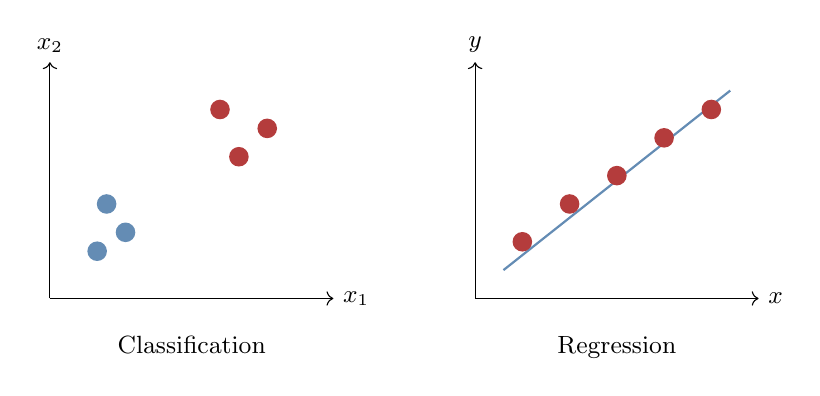
\begin{tikzpicture}[scale=1.2]
% Classification plot
\begin{scope}
\draw[->] (0,0) -- (3,0) node[right] {\small $x_1$};
\draw[->] (0,0) -- (0,2.5) node[above] {\small $x_2$};
\node[circle,fill=softblue,inner sep=2.5pt] at (0.5,0.5) {};
\node[circle,fill=softblue,inner sep=2.5pt] at (0.8,0.7) {};
\node[circle,fill=softblue,inner sep=2.5pt] at (0.6,1.0) {};
\node[circle,fill=softred,inner sep=2.5pt] at (2.0,1.5) {};
\node[circle,fill=softred,inner sep=2.5pt] at (2.3,1.8) {};
\node[circle,fill=softred,inner sep=2.5pt] at (1.8,2.0) {};
\node[below] at (1.5,-0.3) {\small Classification};
\end{scope}

% Regression plot
\begin{scope}[xshift=4.5cm]
\draw[->] (0,0) -- (3,0) node[right] {\small $x$};
\draw[->] (0,0) -- (0,2.5) node[above] {\small $y$};
\draw[softblue,thick] (0.3,0.3) -- (2.7,2.2);
\node[circle,fill=softred,inner sep=2.5pt] at (0.5,0.6) {};
\node[circle,fill=softred,inner sep=2.5pt] at (1.0,1.0) {};
\node[circle,fill=softred,inner sep=2.5pt] at (1.5,1.3) {};
\node[circle,fill=softred,inner sep=2.5pt] at (2.0,1.7) {};
\node[circle,fill=softred,inner sep=2.5pt] at (2.5,2.0) {};
\node[below] at (1.5,-0.3) {\small Regression};
\end{scope}
\end{tikzpicture}
\end{center}
\end{frame}

\begin{frame}{Unsupervised Learning: Clustering vs Dimensionality Reduction}
\small
\begin{columns}[T]
\column{0.48\textwidth}
\textbf{Clustering}
\begin{itemize}
\item Group similar data points
\item No predefined labels
\item Discover natural groupings
\end{itemize}

\vspace{0.1cm}
\textbf{Examples:}
\begin{itemize}
\item Customer segmentation
\item Document organization
\item \textcolor{pythonblue}{Grouping similar bridge designs}
\item \textcolor{pythonblue}{Identifying failure patterns}
\end{itemize}

\column{0.48\textwidth}
\textbf{Dimensionality Reduction}
\begin{itemize}
\item Reduce number of features
\item Preserve important information
\item Visualization \& compression
\end{itemize}


\textbf{Examples:}
\begin{itemize}
\item Image compression
\item Feature extraction
\item \textcolor{pythonblue}{Compress sensor data streams}
\item \textcolor{pythonblue}{Visualize high-D material properties}
\end{itemize}
\end{columns}
\end{frame}

\begin{frame}{Visualizing Clustering and Dimensionality Reduction}
\begin{center}
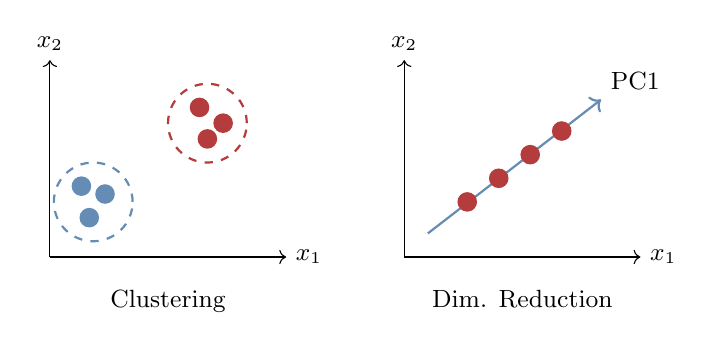
\begin{tikzpicture}[scale=1.0]
% Clustering
\begin{scope}
\draw[->] (0,0) -- (3,0) node[right] {\small $x_1$};
\draw[->] (0,0) -- (0,2.5) node[above] {\small $x_2$};
\node[circle,fill=softblue,inner sep=2.5pt] at (0.5,0.5) {};
\node[circle,fill=softblue,inner sep=2.5pt] at (0.7,0.8) {};
\node[circle,fill=softblue,inner sep=2.5pt] at (0.4,0.9) {};
\node[circle,fill=softred,inner sep=2.5pt] at (2.0,1.5) {};
\node[circle,fill=softred,inner sep=2.5pt] at (2.2,1.7) {};
\node[circle,fill=softred,inner sep=2.5pt] at (1.9,1.9) {};
\draw[dashed,softblue,thick] (0.55,0.7) circle (0.5cm);
\draw[dashed,softred,thick] (2.0,1.7) circle (0.5cm);
\node[below] at (1.5,-0.3) {\small Clustering};
\end{scope}

% Dim Reduction
\begin{scope}[xshift=4.5cm]
\draw[->] (0,0) -- (3,0) node[right] {\small $x_1$};
\draw[->] (0,0) -- (0,2.5) node[above] {\small $x_2$};
\draw[softblue,thick,->] (0.3,0.3) -- (2.5,2.0);
\node[circle,fill=softred,inner sep=2.5pt] at (0.8,0.7) {};
\node[circle,fill=softred,inner sep=2.5pt] at (1.2,1.0) {};
\node[circle,fill=softred,inner sep=2.5pt] at (1.6,1.3) {};
\node[circle,fill=softred,inner sep=2.5pt] at (2.0,1.6) {};
\node[below] at (1.5,-0.3) {\small Dim. Reduction};
\node[above right] at (2.5,2.0) {\small PC1};
\end{scope}
\end{tikzpicture}
\end{center}
\end{frame}

\begin{frame}{Machine Learning Workflow}
\small
\textbf{Key Steps:}
\begin{enumerate}
\item \textbf{Data Collection \& Preprocessing:} Gather, clean, normalize data
\item \textbf{Feature Engineering:} Select/create informative features
\item \textbf{Model Selection \& Training:} Choose algorithm, fit to data
\item \textbf{Validation:} Test on unseen data, tune hyperparameters
\item \textbf{Deployment:} Use model in production
\end{enumerate}
\end{frame}

\begin{frame}{Machine Learning Workflow Diagram}
\begin{center}
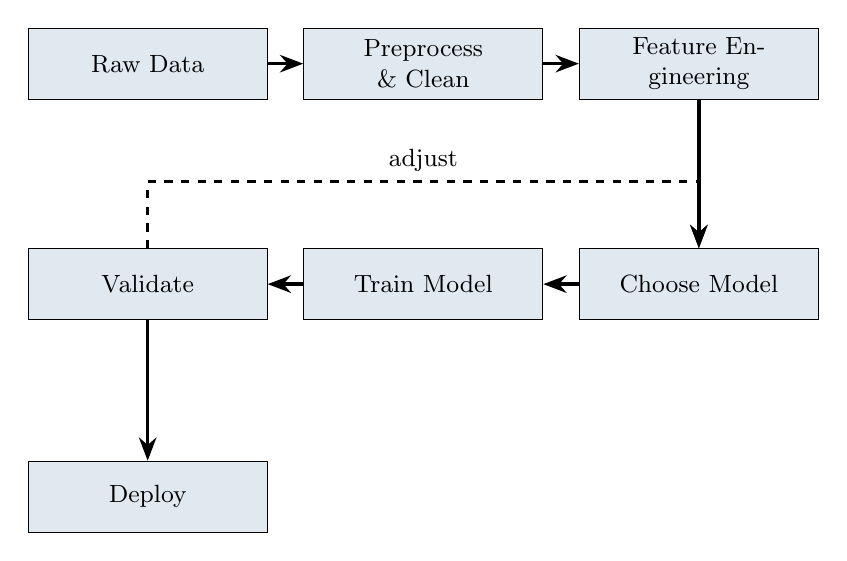
\begin{tikzpicture}[
    node distance=2cm,
    box/.style={rectangle, draw, fill=softblue!20, text width=2.8cm, align=center, minimum height=0.9cm, font=\small},
    arrow/.style={->, >=Stealth, very thick}
]
\node[box] (data) {Raw Data};
\node[box, right of=data, xshift=1.5cm] (preprocess) {Preprocess \& Clean};
\node[box, right of=preprocess, xshift=1.5cm] (features) {Feature Engineering};
\node[box, below of=features, yshift=-0.8cm] (model) {Choose Model};
\node[box, left of=model, xshift=-1.5cm] (train) {Train Model};
\node[box, left of=train, xshift=-1.5cm] (validate) {Validate};
\node[box, below of=data, yshift=-3.5cm] (deploy) {Deploy};

\draw[arrow] (data) -- (preprocess);
\draw[arrow] (preprocess) -- (features);
\draw[arrow] (features) -- (model);
\draw[arrow] (model) -- (train);
\draw[arrow] (train) -- (validate);
\draw[arrow] (validate) -- (deploy);
\draw[arrow, dashed] (validate) -- ++(0,1.3) -| node[near start, above] {\small adjust} (model);
\end{tikzpicture}
\end{center}
\end{frame}

%% ==================== SECTION 2: INTRODUCING SCIKIT-LEARN ====================
\section{Introducing Scikit-Learn}

\begin{frame}[fragile]{What is Scikit-Learn?}
\small
\textbf{Scikit-Learn} is Python's premier machine learning library

\vspace{0.2cm}
\textbf{Key Features:}
\begin{itemize}
\item \textbf{Consistent API:} All models follow the same interface
\item \textbf{Comprehensive:} Classification, regression, clustering, dimensionality reduction
\item \textbf{Well-documented:} Excellent documentation and examples
\item \textbf{Built on NumPy/SciPy:} Fast and efficient
\item \textbf{Open-source:} Free and actively maintained
\end{itemize}

\vspace{0.2cm}
\textbf{Installation:}
\begin{lstlisting}[language=bash, numbers=none, frame=none, backgroundcolor=\color{white}]
pip install scikit-learn
# or
conda install scikit-learn
\end{lstlisting}

\vspace{0.2cm}
\begin{exampleblock}{Why Scikit-Learn?}
Unified interface means learning one model teaches you all models!
\end{exampleblock}
\end{frame}

\begin{frame}{Data Representation in Scikit-Learn}
\small
\textbf{Two fundamental data structures:}

\vspace{0.2cm}
\begin{columns}[T]
\column{0.48\textwidth}
\textbf{1. Features Matrix: } $\X$
\begin{itemize}
\item Shape: $[n_{samples}, n_{features}]$
\item Usually denoted as $\X$
\item Each row: one sample
\item Each column: one feature
\item Typically a 2D NumPy array or pandas DataFrame
\end{itemize}

\column{0.48\textwidth}
\textbf{2. Target Array: } $\y$
\begin{itemize}
\item Shape: $[n_{samples}]$
\item Usually denoted as $\y$
\item Labels (classification) or values (regression)
\item Typically a 1D NumPy array or pandas Series
\end{itemize}
\end{columns}
\end{frame}



\begin{frame}[fragile]{The Estimator API}
\small
\textbf{All Scikit-Learn models follow the same pattern:}

\vspace{0.2cm}
\begin{enumerate}
\item \textbf{Choose a model class} and import it
\item \textbf{Choose hyperparameters} by instantiating the class
\item \textbf{Arrange data} into features matrix $\X$ and target vector $\y$
\item \textbf{Fit the model} to your data with \py{.fit()}
\item \textbf{Apply the model} with \py{.predict()} or \py{.transform()}
\end{enumerate}

\vspace{0.2cm}
\textbf{Universal Interface:}
\begin{lstlisting}
from sklearn.some_module import SomeModel

# 1. Choose model and hyperparameters
model = SomeModel(hyperparameter1=value1,
                  hyperparameter2=value2)

# 2. Fit to data
model.fit(X, y)

# 3. Predict on new data
predictions = model.predict(X_new)
\end{lstlisting}
\end{frame}

\begin{frame}[fragile]{Example: Simple Linear Regression}
\small
\textbf{Problem:} Predict concrete strength from water-cement ratio
\begin{lstlisting}
import numpy as np
from sklearn.linear_model import LinearRegression

# Generate sample data (water-cement ratio vs strength)
X = np.array([[0.4], [0.45], [0.5], [0.55], [0.6], [0.65]])
y = np.array([45, 40, 35, 30, 25, 20])  # Strength in MPa

# 1. Choose model
model = LinearRegression()

# 2. Fit model
model.fit(X, y)

# 3. Make predictions
X_new = np.array([[0.48], [0.58]])
predictions = model.predict(X_new)

print(f"Predictions: {predictions}")
print(f"Slope: {model.coef_[0]:.2f}")
print(f"Intercept: {model.intercept_:.2f}")
\end{lstlisting}
\begin{exampleblock}{Output}
\texttt{Predictions: [37.5  27.5]  |  Slope: -50.00  |  Intercept: 65.00}
\end{exampleblock}
\end{frame}

\begin{frame}[fragile]{Example: Classification with Iris Dataset}
\small
\textbf{Problem:} Classify iris flowers based on petal/sepal measurements
\begin{lstlisting}
from sklearn.datasets import load_iris
from sklearn.model_selection import train_test_split
from sklearn.neighbors import KNeighborsClassifier

# Load data
iris = load_iris()
X, y = iris.data, iris.target

# Split data: 80% training, 20% testing
X_train, X_test, y_train, y_test = train_test_split(
    X, y, test_size=0.2, random_state=42)

# Create and train model (k=3 nearest neighbors)
model = KNeighborsClassifier(n_neighbors=3)
model.fit(X_train, y_train)

# Evaluate accuracy
accuracy = model.score(X_test, y_test)
print(f"Test Accuracy: {accuracy:.2%}")
\end{lstlisting}

\begin{exampleblock}{Civil Engineering Analogy}
Replace iris measurements with soil properties (grain size, moisture, density) to classify soil types (clay, silt, sand).
\end{exampleblock}
\end{frame}

\begin{frame}[fragile]{Unsupervised Learning: PCA Example}
\small
\textbf{Principal Component Analysis (PCA):} Reduce dimensionality while preserving variance

\begin{lstlisting}
from sklearn.decomposition import PCA
from sklearn.datasets import load_iris

# Load high-dimensional data (4 features)
iris = load_iris()
X = iris.data  # Shape: (150, 4)

# Reduce to 2 dimensions for visualization
pca = PCA(n_components=2)
X_reduced = pca.fit_transform(X)  # Shape: (150, 2)

# How much variance is explained?
print(f"Explained variance: {pca.explained_variance_ratio_}")
print(f"Total: {sum(pca.explained_variance_ratio_):.2%}")
\end{lstlisting}

\begin{exampleblock}{Engineering Application}
Compress multi-sensor structural health monitoring data from 100 sensors to 5 principal components, retaining 95\% of information.
\end{exampleblock}
\end{frame}

\begin{frame}[fragile]{Unsupervised Learning: K-Means Clustering}
\small
\textbf{K-Means:} Group data into $k$ clusters

\begin{lstlisting}
from sklearn.cluster import KMeans
import numpy as np

# Sample data: structural damage measurements
X = np.array([[1, 2], [1.5, 1.8], [5, 8],
              [8, 8], [1, 0.6], [9, 11]])

# Create 2 clusters
kmeans = KMeans(n_clusters=2, random_state=42)
kmeans.fit(X)

# Get cluster labels
labels = kmeans.labels_
print(f"Cluster assignments: {labels}")

# Get cluster centers
centers = kmeans.cluster_centers_
print(f"Cluster centers:\n{centers}")
\end{lstlisting}

\begin{exampleblock}{Civil Engineering Application}
Cluster bridge inspection data to identify structures with similar damage patterns for targeted maintenance strategies.
\end{exampleblock}
\end{frame}

%% ==================== SECTION 3: MODEL VALIDATION ====================
\section{Hyperparameters and Model Validation}

\begin{frame}{Why Model Validation?}
\small
\textbf{The Fundamental Problem:}
\begin{itemize}
\item We want models that \textbf{generalize} to new, unseen data
\item Simply fitting training data is not enough
\item Need to estimate performance on future data
\end{itemize}

\vspace{0.2cm}
\begin{alertblock}{Common Mistake: Training on Test Data}
\textbf{WRONG:} Evaluate model on the same data used for training\\
\textbf{Result:} Overly optimistic performance estimates
\end{alertblock}

\vspace{0.2cm}
\textbf{Solution:} Hold out a separate \textbf{test set}
\end{frame}

\begin{frame}{Train-Test Split Visualization}
\begin{center}
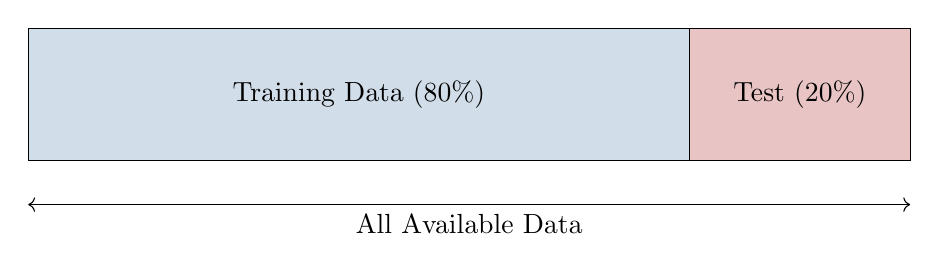
\begin{tikzpicture}[scale=1.4]
\draw[fill=softblue!30] (0,0) rectangle (6,1.2);
\draw[fill=softred!30] (6,0) rectangle (8,1.2);
\node at (3,0.6) {Training Data (80\%)};
\node at (7,0.6) {Test (20\%)};
\draw[<->] (0,-0.4) -- (8,-0.4) node[midway,below] {All Available Data};
\end{tikzpicture}
\end{center}
\end{frame}

\begin{frame}[fragile]{Train-Test Split}
\small
\textbf{Basic Approach:} Split data into training and testing sets
\begin{lstlisting}
from sklearn.model_selection import train_test_split
from sklearn.linear_model import LinearRegression

# Split: 80% train, 20% test
X_train, X_test, y_train, y_test = train_test_split(
    X, y, test_size=0.2, random_state=42)

# Fit on training data only
model = LinearRegression()
model.fit(X_train, y_train)

# Evaluate on test data
train_score = model.score(X_train, y_train)
test_score = model.score(X_test, y_test)

print(f"Training R^2: {train_score:.3f}")
print(f"Test R^2: {test_score:.3f}")
\end{lstlisting}

\vspace{0.05cm}
\begin{block}{Key Points}
\begin{itemize}
\item \py{random\_state}: ensures reproducibility
\item \textbf{Never} use test data during training or hyperparameter tuning
\item Test set estimates performance on unseen data
\end{itemize}
\end{block}
\end{frame}

\begin{frame}{Cross-Validation}
\small
\textbf{Problem with single train-test split:}
\begin{itemize}
\item Performance depends on which samples ended up in test set
\item Wastes data (only 80\% used for training)
\end{itemize}

\vspace{0.2cm}
\textbf{Solution: K-Fold Cross-Validation}

\vspace{0.2cm}
\textbf{Process:}
\begin{enumerate}
\item Split data into $k$ equal parts (folds)
\item Train on $k-1$ folds, test on the remaining fold
\item Repeat $k$ times, each fold used as test set once
\item Average the $k$ performance scores
\end{enumerate}
\end{frame}

\begin{frame}{K-Fold Cross-Validation Diagram}
\begin{center}
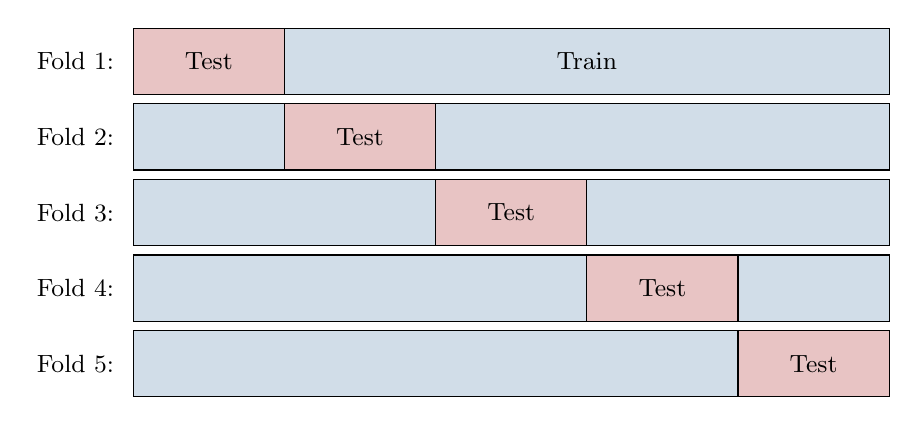
\begin{tikzpicture}[scale=1.2]
% Fold 1
\draw[fill=softred!30] (0,0) rectangle (1.6,0.7);
\draw[fill=softblue!30] (1.6,0) rectangle (8,0.7);
\node[left] at (-0.1,0.35) {\small Fold 1:};
\node at (0.8,0.35) {\small Test};
\node at (4.8,0.35) {\small Train};

% Fold 2
\draw[fill=softblue!30] (0,-0.8) rectangle (1.6,-0.1);
\draw[fill=softred!30] (1.6,-0.8) rectangle (3.2,-0.1);
\draw[fill=softblue!30] (3.2,-0.8) rectangle (8,-0.1);
\node[left] at (-0.1,-0.45) {\small Fold 2:};
\node at (2.4,-0.45) {\small Test};

% Fold 3
\draw[fill=softblue!30] (0,-1.6) rectangle (3.2,-0.9);
\draw[fill=softred!30] (3.2,-1.6) rectangle (4.8,-0.9);
\draw[fill=softblue!30] (4.8,-1.6) rectangle (8,-0.9);
\node[left] at (-0.1,-1.25) {\small Fold 3:};
\node at (4.0,-1.25) {\small Test};

% Fold 4
\draw[fill=softblue!30] (0,-2.4) rectangle (4.8,-1.7);
\draw[fill=softred!30] (4.8,-2.4) rectangle (6.4,-1.7);
\draw[fill=softblue!30] (6.4,-2.4) rectangle (8,-1.7);
\node[left] at (-0.1,-2.05) {\small Fold 4:};
\node at (5.6,-2.05) {\small Test};

% Fold 5
\draw[fill=softblue!30] (0,-3.2) rectangle (6.4,-2.5);
\draw[fill=softred!30] (6.4,-3.2) rectangle (8,-2.5);
\node[left] at (-0.1,-2.85) {\small Fold 5:};
\node at (7.2,-2.85) {\small Test};
\end{tikzpicture}
\end{center}
\end{frame}

\begin{frame}[fragile]{K-Fold Cross-Validation in Scikit-Learn}
\small
\begin{lstlisting}
from sklearn.model_selection import cross_val_score
from sklearn.linear_model import LinearRegression

# Create model
model = LinearRegression()

# Perform 5-fold cross-validation
scores = cross_val_score(model, X, y, cv=5,
                         scoring='r2')

print(f"Cross-validation scores: {scores}")
print(f"Mean R^2: {scores.mean():.3f}")
print(f"Std Dev: {scores.std():.3f}")
\end{lstlisting}

\vspace{0.2cm}
\textbf{Advantages:}
\begin{itemize}
\item More robust performance estimate
\item Uses all data for both training and validation
\item Provides variance estimate (standard deviation)
\end{itemize}

\vspace{0.2cm}
\begin{exampleblock}{Typical Choice}
5-fold or 10-fold cross-validation is standard. Use more folds for small datasets.
\end{exampleblock}
\end{frame}

\begin{frame}{Bias-Variance Tradeoff}
\small
\textbf{Two sources of model error:}

\vspace{0.2cm}
\begin{columns}[T]
\column{0.48\textwidth}
\textbf{Bias (Underfitting)}
\begin{itemize}
\item Model too simple
\item Cannot capture true pattern
\item High training error
\item High test error
\end{itemize}

\vspace{0.1cm}
\textbf{Example:}\\
Linear model for nonlinear data

\column{0.48\textwidth}
\textbf{Variance (Overfitting)}
\begin{itemize}
\item Model too complex
\item Fits noise in training data
\item Low training error
\item High test error
\end{itemize}

\vspace{0.1cm}
\textbf{Example:}\\
High-degree polynomial
\end{columns}

\vspace{0.2cm}
\textbf{Goal:} Find the sweet spot with minimum test error!
\end{frame}

\begin{frame}{Bias-Variance Tradeoff Visualization}
\begin{center}
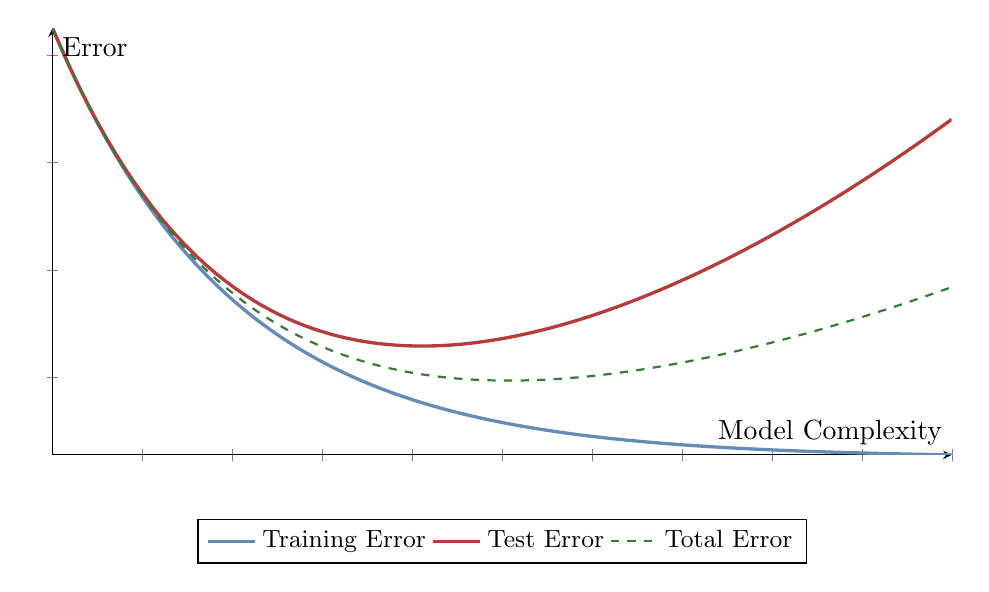
\begin{tikzpicture}
\begin{axis}[
    width=13cm, height=7cm,
    xlabel={Model Complexity},
    ylabel={Error},
    domain=0:10,
    samples=100,
    axis lines=middle,
    xticklabels={},
    yticklabels={},
    legend style={at={(0.5,-0.15)}, anchor=north, legend columns=3, font=\small}
]
\addplot[softblue, very thick] {2.5 + 8*exp(-x/2)};
\addlegendentry{Training Error}
\addplot[softred, very thick] {2.5 + 8*exp(-x/2) + 0.5*x^2/8};
\addlegendentry{Test Error}
\addplot[softgreen, dashed, thick] {2.5 + 8*exp(-x/2) + 0.25*x^2/8};
\addlegendentry{Total Error}
\node[below] at (axis cs:1.5,0) {\small Underfitting};
\node[below] at (axis cs:5,0) {\small Good};
\node[below] at (axis cs:8.5,0) {\small Overfitting};
\end{axis}
\end{tikzpicture}
\end{center}
\end{frame}

\begin{frame}{Validation Curves}
\small
\textbf{Validation Curve:} Plot performance vs. a single hyperparameter

\vspace{0.2cm}
\textbf{Purpose:}
\begin{itemize}
\item Visualize bias-variance tradeoff
\item Select optimal hyperparameter value
\item Diagnose under/overfitting
\end{itemize}
\end{frame}

\begin{frame}{Example Validation Curve}
\begin{center}
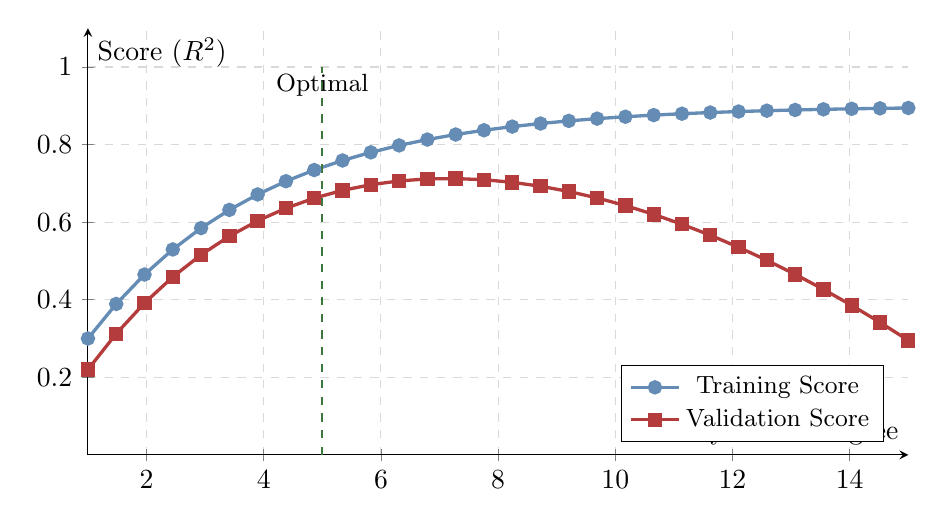
\begin{tikzpicture}
\begin{axis}[
    width=12cm, height=7cm,
    xlabel={Polynomial Degree},
    ylabel={Score ($R^2$)},
    domain=1:15,
    samples=30,
    axis lines=middle,
    ymin=0, ymax=1.1,
    legend style={at={(0.97,0.03)}, anchor=south east, font=\small},
    grid=major,
    grid style={dashed, gray!30}
]
% Training score (always increases)
\addplot[softblue, very thick, mark=*, mark size=2pt] {0.3 + 0.6*(1-exp(-(x-1)/3))};
\addlegendentry{Training Score}
% Validation score (increases then decreases)
\addplot[softred, very thick, mark=square*, mark size=2pt] {0.3 + 0.5*(1-exp(-(x-1)/3)) - 0.05*(x-5)^2/10};
\addlegendentry{Validation Score}
\draw[dashed, softgreen, thick] (axis cs:5,0) -- (axis cs:5,1);
\node[above, font=\small] at (axis cs:5,0.9) {Optimal};
\end{axis}
\end{tikzpicture}
\end{center}
\end{frame}

\begin{frame}[fragile]{Creating Validation Curves}
\small
\begin{lstlisting}
from sklearn.model_selection import validation_curve
from sklearn.linear_model import Ridge
import numpy as np

# Test different regularization strengths
param_range = np.logspace(-4, 4, 10)

train_scores, val_scores = validation_curve(
    Ridge(), X, y,
    param_name='alpha',
    param_range=param_range,
    cv=5,
    scoring='r2'
)

# Average across folds
train_mean = train_scores.mean(axis=1)
val_mean = val_scores.mean(axis=1)

# Find best alpha
best_alpha = param_range[val_mean.argmax()]
print(f"Best alpha: {best_alpha:.4f}")
\end{lstlisting}

\begin{exampleblock}{Engineering Application}
Tune regularization strength when predicting structural response to prevent overfitting to measurement noise.
\end{exampleblock}
\end{frame}

\begin{frame}{Learning Curves}
\small
\textbf{Learning Curve:} Plot performance vs. training set size

\vspace{0.1cm}
\textbf{Purpose:}
\begin{itemize}
\item Diagnose whether more data will help
\item Identify high bias vs. high variance
\end{itemize}

\vspace{0.2cm}
\textbf{Diagnosis:}
\begin{itemize}
\item \textbf{Large gap:} High variance $\rightarrow$ more data or regularization
\item \textbf{Converged low:} High bias $\rightarrow$ more complex model
\end{itemize}
\end{frame}

\begin{frame}{Learning Curves: High Variance vs High Bias}
\begin{center}
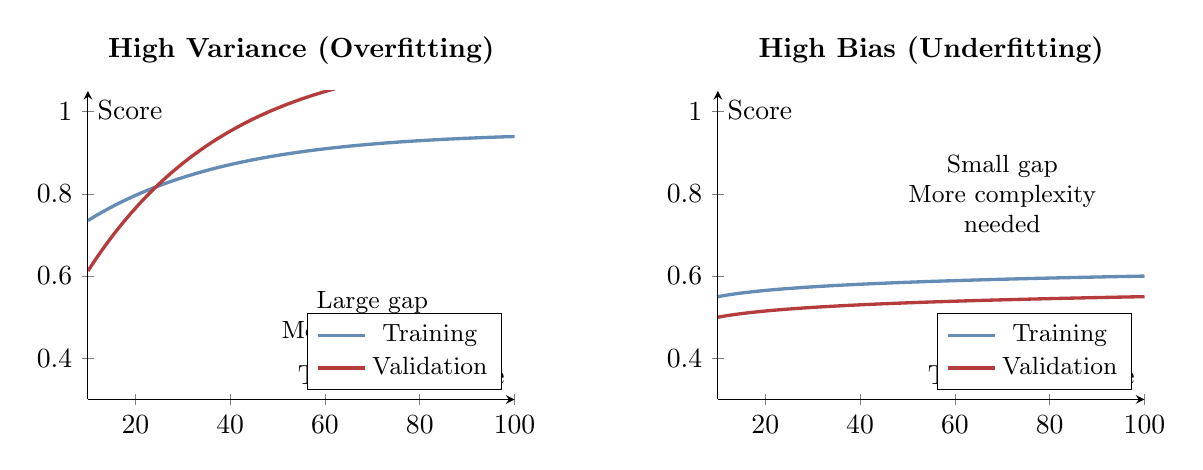
\begin{tikzpicture}
\begin{axis}[
    width=7cm, height=5.5cm,
    xlabel={Training Set Size},
    ylabel={Score},
    domain=10:100,
    samples=50,
    axis lines=middle,
    ymin=0.3, ymax=1.05,
    legend style={at={(0.97,0.03)}, anchor=south east, font=\small},
    title={\textbf{High Variance (Overfitting)}},
    title style={font=\normalsize}
]
\addplot[softblue, very thick] {0.95 - 0.3*exp(-x/30)};
\addlegendentry{Training}
\addplot[softred, very thick] {0.75*(1-exp(-x/30)) + 0.4};
\addlegendentry{Validation}
\node[font=\small, align=center] at (axis cs:70,0.5) {Large gap\\More data helps};
\end{axis}

\begin{axis}[
    xshift=8cm,
    width=7cm, height=5.5cm,
    xlabel={Training Set Size},
    ylabel={Score},
    domain=10:100,
    samples=50,
    axis lines=middle,
    ymin=0.3, ymax=1.05,
    legend style={at={(0.97,0.03)}, anchor=south east, font=\small},
    title={\textbf{High Bias (Underfitting)}},
    title style={font=\normalsize}
]
\addplot[softblue, very thick] {0.55 + 0.05*log10(x/10)};
\addlegendentry{Training}
\addplot[softred, very thick] {0.50 + 0.05*log10(x/10)};
\addlegendentry{Validation}
\node[font=\small, align=center] at (axis cs:70,0.8) {Small gap\\More complexity\\needed};
\end{axis}
\end{tikzpicture}
\end{center}
\end{frame}

\begin{frame}[fragile]{Grid Search for Hyperparameter Tuning}
\small
\textbf{Problem:} Many models have multiple hyperparameters to tune

\vspace{0.2cm}
\textbf{Grid Search:} Try all combinations of hyperparameters

\vspace{0.2cm}
\begin{lstlisting}
from sklearn.model_selection import GridSearchCV
from sklearn.svm import SVC

# Define parameter grid
param_grid = {
    'C': [0.1, 1, 10, 100],
    'gamma': [0.001, 0.01, 0.1, 1],
    'kernel': ['rbf', 'linear']
}

# Create grid search with 5-fold CV
grid = GridSearchCV(SVC(), param_grid, cv=5,
                    scoring='accuracy')

# Fit searches all combinations
grid.fit(X_train, y_train)

print(f"Best parameters: {grid.best_params_}")
print(f"Best CV score: {grid.best_score_:.3f}")

# Use best model for predictions
best_model = grid.best_estimator_
\end{lstlisting}
\end{frame}

%% ==================== SECTION 4: LINEAR REGRESSION ====================
\section{Linear Regression}

\begin{frame}{Linear Regression: The Foundation}
\small
\textbf{Goal:} Fit a linear relationship between features and target

\vspace{0.1cm}
\textbf{Model:}
$$\hat{y} = w_0 + w_1 x_1 + w_2 x_2 + \cdots + w_p x_p = w_0 + \sum_{j=1}^{p} w_j x_j$$

\vspace{0.05cm}
Where: $\hat{y}$ = predicted value, $x_j$ = features, $w_j$ = weights, $w_0$ = intercept

\vspace{0.1cm}
\textbf{Learning Objective:} Find weights that minimize error

$$\text{minimize} \quad \sum_{i=1}^{n} (y_i - \hat{y}_i)^2 = \sum_{i=1}^{n} \left(y_i - w_0 - \sum_{j=1}^{p} w_j x_{ij}\right)^2$$

\begin{exampleblock}{Civil Engineering Example}
Predict concrete compressive strength from: cement content, water ratio, age, aggregate size, etc.
\end{exampleblock}
\end{frame}

\begin{frame}[fragile]{Simple Linear Regression Example}
\small
\begin{lstlisting}
import numpy as np
import matplotlib.pyplot as plt
from sklearn.linear_model import LinearRegression

# Data: Age vs Concrete Strength
age = np.array([3, 7, 14, 28, 56, 90])
strength = np.array([20, 32, 38, 45, 50, 52])

X = age.reshape(-1, 1)
y = strength

# Fit model
model = LinearRegression()
model.fit(X, y)

# Coefficients
print(f"Slope: {model.coef_[0]:.2f}")
print(f"Intercept: {model.intercept_:.2f}")
print(f"R^2: {model.score(X, y):.3f}")

# Predict
age_new = np.array([[21], [42]])
pred = model.predict(age_new)
\end{lstlisting}
\end{frame}

\begin{frame}{Linear Regression Fit Example}
\begin{center}
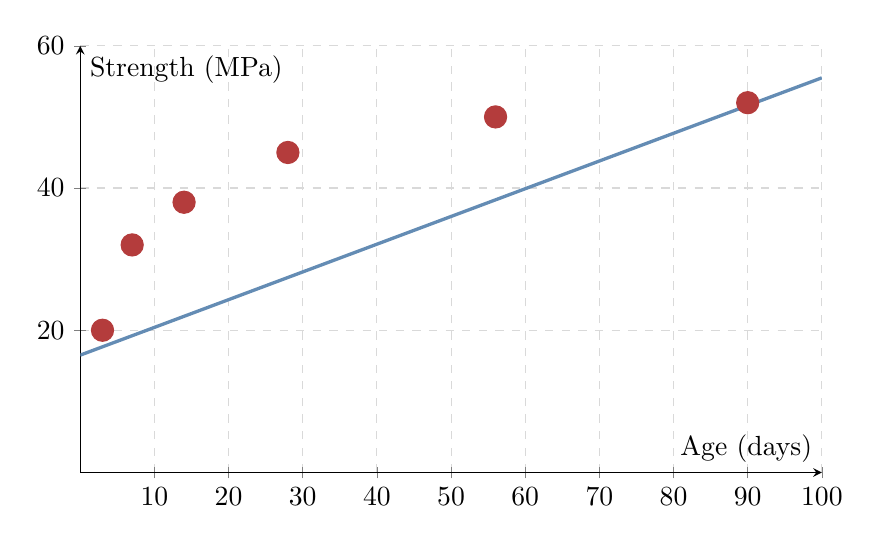
\begin{tikzpicture}
\begin{axis}[
    width=11cm, height=7cm,
    xlabel={Age (days)},
    ylabel={Strength (MPa)},
    axis lines=middle,
    grid=major,
    grid style={dashed, gray!30},
    xmin=0, xmax=100,
    ymin=0, ymax=60
]
\addplot[only marks, mark=*, softred, mark size=4pt] coordinates {
    (3,20) (7,32) (14,38) (28,45) (56,50) (90,52)
};
\addplot[softblue, very thick, domain=0:100] {16.5 + 0.39*x};
\end{axis}
\end{tikzpicture}
\end{center}

\vspace{0.2cm}
\textbf{Interpretation:}
\begin{itemize}
\item Each day adds 0.39 MPa
\item Base strength: 16.5 MPa
\item $R^2 = 0.98$ (good fit)
\end{itemize}
\end{frame}

\begin{frame}{Polynomial Regression}
\small
\textbf{Idea:} Use polynomial features to fit nonlinear relationships

\vspace{0.1cm}
\textbf{Transform:}
$$x \rightarrow [x, x^2, x^3, \ldots, x^d]$$
Then apply linear regression: $\hat{y} = w_0 + w_1 x + w_2 x^2 + \cdots + w_d x^d$

\vspace{0.2cm}
\begin{alertblock}{Warning}
Higher degree $\rightarrow$ more flexibility $\rightarrow$ risk of overfitting!
\end{alertblock}
\end{frame}

\begin{frame}{Polynomial Regression: Degree Comparison}
\begin{center}
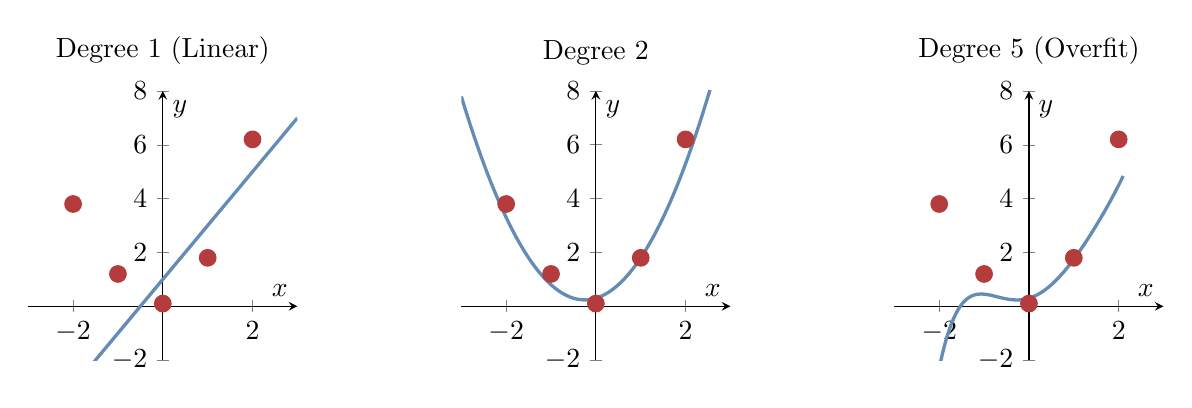
\begin{tikzpicture}
\begin{axis}[
    width=5cm, height=5cm,
    xlabel={$x$},
    ylabel={$y$},
    axis lines=middle,
    title={Degree 1 (Linear)},
    title style={font=\normalsize},
    xmin=-3, xmax=3,
    ymin=-2, ymax=8
]
\addplot[only marks, mark=*, softred, mark size=3pt] coordinates {
    (-2,3.8) (-1,1.2) (0,0.1) (1,1.8) (2,6.2)
};
\addplot[softblue, very thick, domain=-3:3] {2*x + 1};
\end{axis}

\begin{axis}[
    xshift=5.5cm,
    width=5cm, height=5cm,
    xlabel={$x$},
    ylabel={$y$},
    axis lines=middle,
    title={Degree 2},
    title style={font=\normalsize},
    xmin=-3, xmax=3,
    ymin=-2, ymax=8
]
\addplot[only marks, mark=*, softred, mark size=3pt] coordinates {
    (-2,3.8) (-1,1.2) (0,0.1) (1,1.8) (2,6.2)
};
\addplot[softblue, very thick, domain=-3:3, samples=100] {x^2 + 0.5*x + 0.3};
\end{axis}

\begin{axis}[
    xshift=11cm,
    width=5cm, height=5cm,
    xlabel={$x$},
    ylabel={$y$},
    axis lines=middle,
    title={Degree 5 (Overfit)},
    title style={font=\normalsize},
    xmin=-3, xmax=3,
    ymin=-2, ymax=8
]
\addplot[only marks, mark=*, softred, mark size=3pt] coordinates {
    (-2,3.8) (-1,1.2) (0,0.1) (1,1.8) (2,6.2)
};
\addplot[softblue, very thick, domain=-2.1:2.1, samples=100] {
    0.3 + 0.5*x + x^2 + 0.1*x^3 - 0.2*x^4 + 0.05*x^5
};
\end{axis}
\end{tikzpicture}
\end{center}
\end{frame}

\begin{frame}[fragile]{Polynomial Features in Scikit-Learn}
\small
\begin{lstlisting}
from sklearn.preprocessing import PolynomialFeatures
from sklearn.linear_model import LinearRegression
from sklearn.pipeline import make_pipeline

# Original data
X = np.array([[x] for x in range(10)])
y = np.array([1, 3, 2, 5, 7, 8, 8, 9, 10, 12])

# Create polynomial regression pipeline
# Degree 3: [1, x, x^2, x^3]
model = make_pipeline(
    PolynomialFeatures(degree=3),
    LinearRegression()
)

# Fit and predict
model.fit(X, y)
y_pred = model.predict(X)

# Evaluate
r2 = model.score(X, y)
print(f"R^2 score: {r2:.3f}")
\end{lstlisting}

\vspace{0.1cm}
\textbf{Pipeline:} Chains transformations automatically!
\end{frame}

\begin{frame}{Regularization: Controlling Complexity}
\small
\textbf{Problem:} Complex models overfit to training data

\vspace{0.2cm}
\textbf{Solution:} Add penalty for large coefficients

\vspace{0.2cm}
\begin{columns}[T]
\column{0.48\textwidth}
\textbf{Ridge Regression (L2)}
$$\text{minimize} \sum_{i=1}^{n} (y_i - \hat{y}_i)^2 + \alpha \sum_{j=1}^{p} w_j^2$$

\begin{itemize}
\item Shrinks coefficients
\item Keeps all features
\item $\alpha$: regularization strength
\end{itemize}

\column{0.48\textwidth}
\textbf{Lasso Regression (L1)}
$$\text{minimize} \sum_{i=1}^{n} (y_i - \hat{y}_i)^2 + \alpha \sum_{j=1}^{p} |w_j|$$

\begin{itemize}
\item Shrinks some to exactly zero
\item Performs feature selection
\item $\alpha$: regularization strength
\end{itemize}
\end{columns}

\vspace{0.2cm}
\textbf{Key:} Larger $\alpha$ $\rightarrow$ stronger regularization $\rightarrow$ simpler model
\end{frame}

\begin{frame}{Effect of Regularization on Coefficients}
\begin{center}
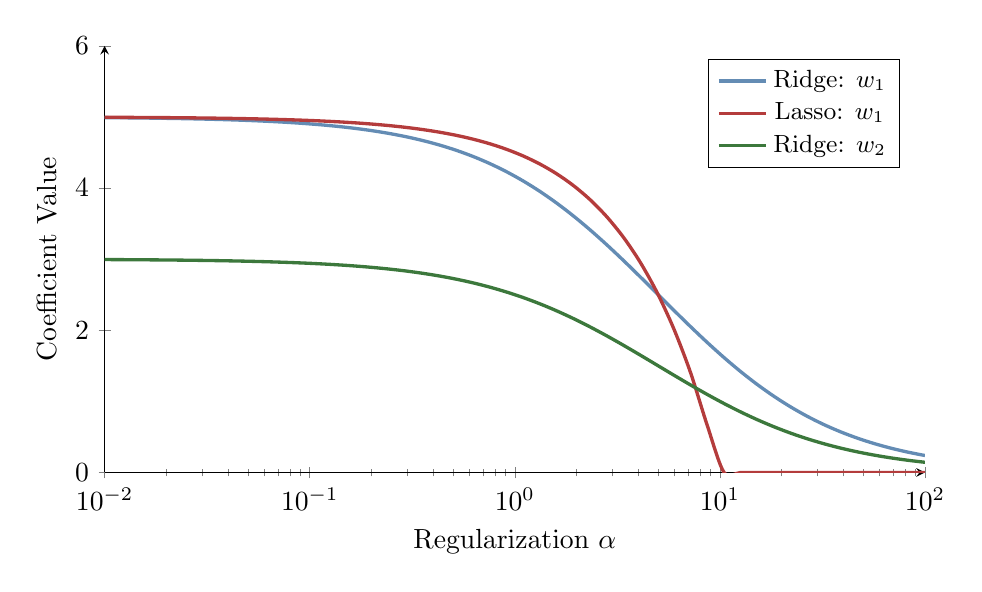
\begin{tikzpicture}
\begin{axis}[
    width=12cm, height=7cm,
    xlabel={Regularization $\alpha$},
    ylabel={Coefficient Value},
    xmode=log,
    axis lines=left,
    legend style={at={(0.97,0.97)}, anchor=north east, font=\small},
    xmin=0.01, xmax=100,
    ymin=0, ymax=6,
    domain=0.01:100,
    samples=50
]
\addplot[softblue, very thick, smooth] {5/(1+0.2*x)};
\addlegendentry{Ridge: $w_1$}
\addplot[softred, very thick, smooth] {max(0, 5-0.5*x)};
\addlegendentry{Lasso: $w_1$}
\addplot[softgreen, very thick, smooth] {3/(1+0.2*x)};
\addlegendentry{Ridge: $w_2$}
\end{axis}
\end{tikzpicture}
\end{center}
\end{frame}

\begin{frame}[fragile]{Ridge and Lasso in Scikit-Learn}
\small
\begin{lstlisting}
from sklearn.linear_model import Ridge, Lasso

# Ridge Regression (L2)
ridge = Ridge(alpha=1.0)  # Try 0.1, 1.0, 10.0
ridge.fit(X_train, y_train)
ridge_score = ridge.score(X_test, y_test)

# Lasso Regression (L1)
lasso = Lasso(alpha=0.1)
lasso.fit(X_train, y_train)
lasso_score = lasso.score(X_test, y_test)

# Compare coefficients
print(f"Ridge coefficients: {ridge.coef_}")
print(f"Lasso coefficients: {lasso.coef_}")
print(f"Non-zero Lasso features: {np.sum(lasso.coef_ != 0)}")
\end{lstlisting}

\vspace{0.2cm}
\begin{exampleblock}{When to Use Which?}
\textbf{Ridge:} When all features are potentially relevant\\
\textbf{Lasso:} When you want automatic feature selection
\end{exampleblock}
\end{frame}

\begin{frame}{Real-World Example: Bicycle Traffic Prediction}
\small
\textbf{Problem:} Predict daily bicycle traffic on Seattle's Fremont Bridge

\vspace{0.2cm}
\textbf{Features:}
\begin{itemize}
\item Temperature, precipitation
\item Day of week, month
\item Holiday indicator
\item Hour of day (if hourly data)
\end{itemize}

\vspace{0.2cm}
\textbf{Approach:}
\begin{enumerate}
\item Feature engineering: add polynomial features for temperature
\item Add interaction terms (e.g., temp × weekend)
\item Use Ridge regression to prevent overfitting
\item Validate with cross-validation
\end{enumerate}


\end{frame}

%% ==================== SECTION 5: SUMMARY ====================
\section{Summary and Next Steps}

\begin{frame}{Key Takeaways}
\small
\textbf{1. Machine Learning Fundamentals}
\begin{itemize}
\item Supervised (classification, regression) vs Unsupervised (clustering, dim reduction)
\item Data-driven approach to building predictive models
\end{itemize}

\vspace{0.2cm}
\textbf{2. Scikit-Learn Workflow}
\begin{itemize}
\item Consistent API: \py{fit()}, \py{predict()}, \py{transform()}
\item Data representation: features matrix $\X$, target vector $\y$
\end{itemize}

\vspace{0.2cm}
\textbf{3. Model Validation}
\begin{itemize}
\item Never evaluate on training data
\item Use train-test split or cross-validation
\item Understand bias-variance tradeoff
\end{itemize}

\vspace{0.2cm}
\textbf{4. Linear Regression}
\begin{itemize}
\item Foundation for many ML algorithms
\item Polynomial features for nonlinearity
\item Regularization (Ridge/Lasso) prevents overfitting
\end{itemize}
\end{frame}

\begin{frame}{Civil Engineering Applications}
\small
\textbf{Machine Learning is transforming civil engineering:}

\vspace{0.2cm}
\begin{enumerate}
\item \textbf{Structural Health Monitoring}
   \begin{itemize}
   \item Classify damage types from sensor data
   \item Predict remaining service life
   \end{itemize}

\item \textbf{Material Science}
   \begin{itemize}
   \item Predict concrete/steel properties from composition
   \item Optimize mix designs
   \end{itemize}

\item \textbf{Traffic \& Transportation}
   \begin{itemize}
   \item Traffic flow prediction and optimization
   \item Route planning and demand forecasting
   \end{itemize}

\item \textbf{Construction Management}
   \begin{itemize}
   \item Project cost and duration estimation
   \item Risk assessment and safety prediction
   \end{itemize}

\item \textbf{Environmental Engineering}
   \begin{itemize}
   \item Water quality prediction
   \item Climate impact assessment
   \end{itemize}
\end{enumerate}
\end{frame}

\begin{frame}{Next Steps in Machine Learning}
\small
\textbf{Coming in Week 8:}
\begin{itemize}
\item \textbf{Naive Bayes:} Probabilistic classification
\item \textbf{Support Vector Machines:} Maximum-margin classifiers
\item \textbf{Decision Trees \& Random Forests:} Ensemble methods
\item \textbf{Clustering:} K-Means, hierarchical clustering
\item \textbf{Dimensionality Reduction:} PCA deep dive
\end{itemize}

\vspace{0.3cm}
\textbf{Practice Resources:}
\begin{itemize}
\item \textbf{Scikit-Learn Documentation:} \url{https://scikit-learn.org}
\item \textbf{Kaggle:} Real-world datasets and competitions
\item \textbf{Course Notebooks:} Hands-on examples in repository
\end{itemize}


\end{frame}

\begin{frame}{Questions?}
\begin{center}
\vspace{1cm}
{\Large Thank you!}

\vspace{1cm}
\textbf{Dr. Eyuphan Koc}\\
\texttt{eyuphan.koc@bogazici.edu.tr}

\vspace{1cm}
\textit{Office Hours: By appointment}

\vspace{0.5cm}
\small
Next Lecture: Advanced ML Algorithms\\
(Naive Bayes, SVM, Random Forests)
\end{center}
\end{frame}

\end{document}
